\documentclass[letterpaper,10pt]{article}
\usepackage{graphicx}
\usepackage{listings}
\usepackage{fullpage}
\usepackage{fixltx2e}
\usepackage{multirow}
\usepackage{amssymb,amsmath}
\usepackage{mathtools}
\usepackage{bm}
\usepackage[hyperfootnotes=false]{hyperref}
\usepackage{url}
\usepackage{subfig}
\usepackage{relsize}
\usepackage{enumitem}
\usepackage{fancyhdr}
\usepackage{framed}
\setlength{\headheight}{14pt}
\pagestyle{fancy}
\headsep = 20pt

% Lineskip mods
\linespread{1.0}
\setlength{\parskip}{0.5\baselineskip}
\setlength{\parindent}{0pt}
\newlength\docparskip
\parskip=6pt
\setlength{\docparskip}{\parskip}
\renewcommand{\arraystretch}{1.085}
\usepackage{xcolor}
\lstset{basicstyle=\ttfamily,
  showstringspaces=false,
  commentstyle=\color{red},
  keywordstyle=\color{blue}
}
\begin{document}

\fancyhf{}
\fancyhead[L]{AME 60614: Numerical Methods}
\fancyhead[R]{Qihao Zhuo: Problem Set 3}
\fancyfoot[C]{\thepage}

\thispagestyle{plain}
\begin{center}
  \large
  \textbf{AME 60614: Numerical Methods} \\
  \textbf{Fall 2021} \\
  \vspace{0.5em}
  \textbf{Problem Set 3} \\
  \vspace{1em}
  Qihao Zhuo
\end{center}

\vspace{1.5em}

\section{Modified Wavenumber Analysis}\label{sec1}
\begin{align*}
  \frac{d\phi_j}{dt}&=\frac{\alpha}{\Delta x^2}\left(-\phi_{j+3}+4\phi_{j+2}-5\phi_{j+1}+2\phi_j\right)\\
  \phi_j &= \psi(t)e^{ikj}
\end{align*}

%\begin{figure}[h]
%  \centering
%  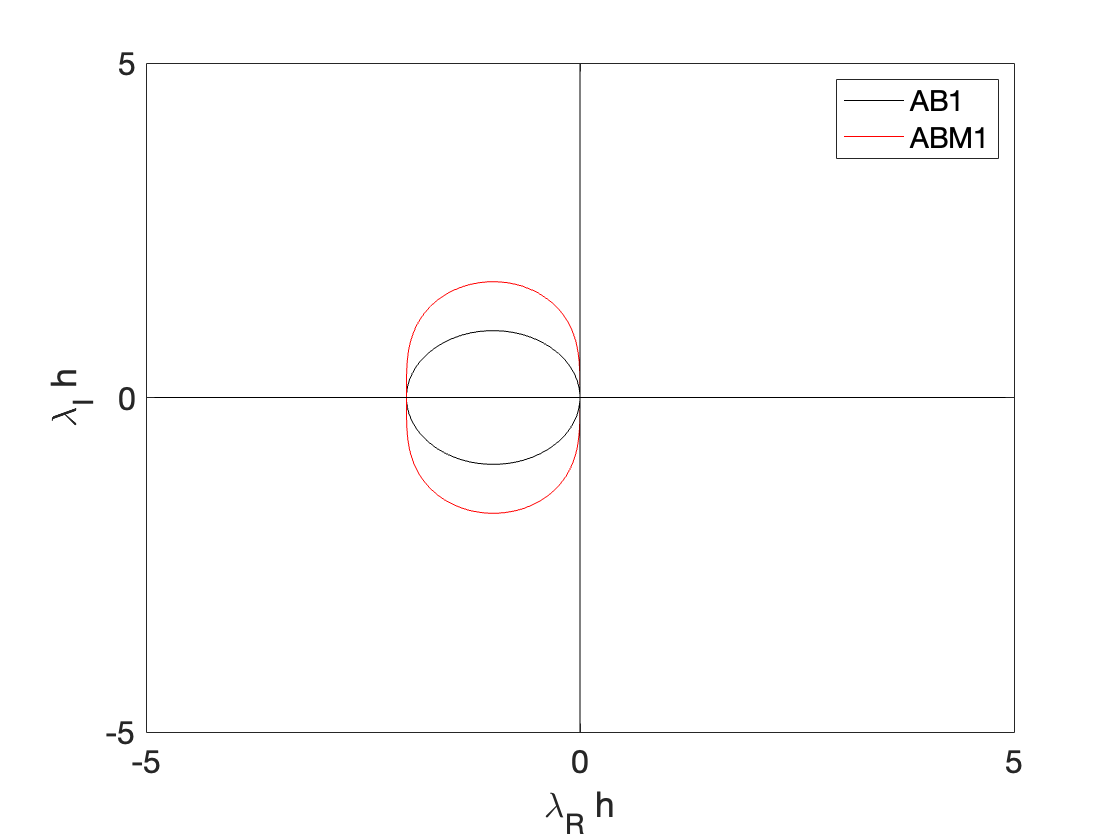
\includegraphics[width=0.5\textwidth]{p1_1.png}
%  \caption{Linear stability diagram after the first corretor step. }
%  \label{fig1_1}
%\end{figure}
\end{document}